\documentclass[a4paper,11pt]{article}
\usepackage[francais]{babel}
\usepackage[T1]{fontenc}
\usepackage[utf8]{inputenc}
\usepackage{graphicx}
\usepackage{color}

\begin {document}

\begin {figure}

\includegraphics[width=0.3\textwidth]{logolemansU.png}
\hspace{150pt}

\includegraphics[width=0.3\textwidth] {logo_ic2.png}
\end {figure}

\title {\textbf {\color {blue} Le Mans Université}\color{black}
\\  Licence Informatique  \textit {2ème année}
\\ Module Conduite de Projet
 \\ \textbf {Projet Hordes}}
\author{Eric Tan - Younès Touffahi - Benjamin Rondeau}
% \author{\href{mailto: eric.tan.etu@univ-lemans.fr} {younes.touffahi.etu@univ-lemans.fr} {benjamin.rondeau.etu@univ-lemans.fr}}
\date{\today}
\maketitle

\newpage

\tableofcontents

\newpage

\section {Introduction}
Vous avez envie de découvrir ou redécouvrir le jeu en ligne nommé Hordes sans être obligé de jouer tous les jours mais plutôt en jouant une partie rapide ?

C’est en effet ce que nous avons tenté de vous proposer avec notre revisite de ce jeu en langage c avec Touffahi Younes, Tan Éric et Rondeau Benjamin.

Pour résumer le jeu Hordes, nous pouvons dire que c’est un jeu de survie en coopération.
Hordes est en effet un jeu qui se joue à plusieurs dont le but est de survivre le plus de jours possibles, en temps réel, dans une ville attaquée par des zombies chaque nuit à minuit. Nous avons opté pour une version plus courte où les zombies attaquent toutes les dix minutes car c’est un peu plus que le temps que nous passons chaque jour à jouer dans le vrai jeu. Chaque joueur a donc 10 minutes pour faire toutes les actions qui lui sont possibles. Le joueur a en effet un inventaire composé de 4 place pour entreposer des objets, des points d’action (PA) au rang de six qui se renouvellent chaque jour si nous sommes en bonne santé et que nous ne sommes pas morts évidemment. Le joueur dispose aussi de différents états comme assoiffé, drogué, blessé, … 

Pour dépenser ses points d’action, le joueur a une interface avec six lieux. Il y a la Maison qui est le coin personnel du joueur, il peut y stocker quatre objets en plus de son inventaire, il peut améliorer sa maison et peut faire des actions spéciales comme manger s’il a ce qu’il faut sur lui ou dans sa maison. Le Puit est le second lieu de l’interface, son seul but est de permettre au joueur de récupérer une ration d’eau chaque jour même s’il est nécessaire de boire qu’une fois tous les deux jours. Ensuite nous avons la banque qui permet de stocker tous les objets de la ville, nous pouvons déposer ou prendre des objets. Par la suite nous avons la catégorie Citoyens qui permet de lister les citoyens, nous avons décidés de ne pas la faire car elle a peu d’utilité dans notre cas car notre version est un jeu qui se joue plutôt entre amis en LAN, on sait donc qui sont les personnes présentes. La quatrième partie est le Chantier qui permet grâce à nos points d’action et à certains objets de la banque d’augmenter les défenses de la ville. L’avant dernière partie est l’Atelier qui permet de transformer certains objets présents dans la banque en d’autres en utilisant nos points d’action. La dernière partie de l’interface est la Grande porte qui permet de sortir de la ville et de se déplacer sur des cases en utilisant des points d’action et fouiller les zones pour trouver des objets pour le reste de la ville et de les ramener grâce à son inventaire. 


\newpage


\section {Organisation du travail}
Le travail a été réparti ainsi :
\\
\\
Eric :
\\
– Boucle de jeu : génération de zombies, défilement des jours, attaque de la ville et mort des joueurs.
\\
– Joueur : Implémenter le joueur avec un pseudo, un inventaire limité à quatre objets, le nombre de points d'actions disponibles, et l'état de santé du joueur.
\\
– Implémentation de bâtiments : La maison(gérer l'inventaire du joueur et ses points d'actions), le puits ( Pour que le joueur puisse récupérer des points d'actions).
\\
– Réseau : Permettre aux joueurs de pouvoir joueur à plusieurs sur un réseau local.
\\
\\
Younès :
\\
– Objets : Implémentation des objets avec leurs différentes caractéristiques, et leurs catégories .
\\
– Implémentation de bâtiments : La banque ( Permettre aux joueurs de partager les objets trouvés en dehors de la ville et ceux fabriqués à l'atelier), l'atelier ( Permet d'utiliser des objets composants provenant de la banque afin de les assembler et créer des matériaux utilisables au chantier), et le chantier(bâtiment de création de structure de défense afin de contrer l'attaque de zombie).
\\
\\
Benjamin :
\\
– Carte : Création de la carte représentant le jeu en dehors de la ville, génération de zombies et d'objets. Implémentation des déplacements du joueurs sur la carte.
\\
\\
Travail commun :
\\
Création du makefile, actions du jeu ( utiliser un objet, déposer un objet, prendre un objet) et enfin l'affichage terminal.
\\
\\
Outils de travail utilisés :
\\
– Github pour pouvoir partager les différents modules et travailler en commun.
\\
– Discord afin de pouvoir discuter à propos du projet en texte ou en vocal.

\newpage

\section {Conception}

\subsection{Choix et Enjeux}
Le premier enjeu majeur du projet est de créer un jeu Hordes beaucoup plus rapide, nous avons choisis de retirer certaine règles, car dans le jeu original, un tour de jeu équivaut à 24 heures en temps réel et le temps de jeu par utilisateur se résume en moyenne à 30 minutes par tour. L'objectif est donc de réduire ce temps de jeu colossal, afin d'obtenir au final 10 minutes pour un tour de jeu.
\\
La génération de zombie à été défini de façon à ce que les joueurs ne soit pas en difficulté selon leurs nombres, de plus le nombres de zombies devient suffisamment important pour que la partie se termine rapidement.
\\
En ce qui concerne le joueur, certains états du jeu original tel que l'infection ont été retirés car cela ralenti le jeu. Par exemple l'état d'infection est la suite d'un autre état celui de blessé, le joueur succombe de ses blessures au bout de 2 tours, l'infection repousse encore à deux tours la mort du joueur et demande des ressources plus rares que celles nécessaire pour une blessure.
\\
Certains bâtiments du jeu original ne sont pas présents car soit cela pouvait demander trop de temps de développement, ou cela ne présenter pas un grand intérêt au niveau de la jouabilité.
\\
Le jeu original possède une grande porte qui pouvait être fermé ou ouverte. Le problème est que si une personne décide de fermer la porte sachant que d'autres personnes se trouvent encore dans la carte, ces joueurs étaient condamnés à mourir car incapable d'ouvrir la porte depuis l'extérieur.
\\
\\
Le second enjeu majeur du projet est de faire en priorité un jeu en réseau, au détriment de l'interface graphique à l'aide de la SDL. Le but du jeu est de survivre, survivre seul est plus complexe que survivre à plusieurs. La construction de défenses nécessite beaucoup de points d'actions, le meilleur moyen au joueur de trouver ces points d'actions et d'avoir de nombreux compagnons de jeu.
\\
La mise en place d'un forum dans le jeu a été retirer, la raison est que le jeu se destine à des parties en LAN, soit à proximité des autres joueurs. L'interaction en vocal suffit est permet une meilleur expérience de jeu et économise un gain de temps en  développement.
\\
Le réseau permettra aux joueurs de partager leurs ressources, par le biais de la banque, ainsi chaque joueur pourra contribuer à la survie des autres, ou à sa survie personnelle.

\newpage

\subsection{Cahier des charges}
Nous allons ici établir les différents aspects du jeu que nous avons pris en compte pour reproduire le jeu en langage C. Commençons par la partie visuel :
\\
\\
Le joueur voit un menu qui correspond aux différentes actions qu'il est capable de faire, il voit aussi sa barre d'inventaire qui peut contenir jusqu'à quatre objets ainsi que son état de santé et le nombre de points d'actions qu'il possède. Chaque option du menu correspond à une zone de la ville.
\\
\\
Le joueur a plusieurs états de santé qui affectent en bien ou en mal ses actions :
\\
- La fatigue, le joueur n'a plus de points d'actions, il est impossible alors de faire des actions consommant des points d'actions.
\\    
- La soif, le joueur a besoin de boire sous peine de mourrir de déshydratation.
\\    
- L'état rassasié, indique que vous avez bu et/ou manger, donc répéter ces actions ne permet plus de récupérer des points d'actions.
\\    
- La blessure, le joueur doit se soigner avant qu'il ne succombe à celle-ci, généralement une personne blessée meurt en deux jours.
\\    
- Drogué(e), le joueur utilisé des substances illicites qui permettent de surmonter les états de fatigue, soif et de blessure. Cependant il ne faut pas abusé des drogues sinon le joueur tombe dans la dépendance.
\\    
- Clair, le joueur n'a pas consommé de drogue.
\\    
- Immunisé, le joueur a consommé un médicament qui permet de guérir de ses blessures.
\\
\\
En dehors de la ville, les actions du joueur sont différentes. Tout comme dans la ville, le joueur voit sa barre d'inventaire, ses points d'actions et son état de santé. Cependant il voit à la place du menu une carte lui montrant la position de la ville et la sienne. Il a aussi accès à d'autres actions comme se déplacer sur la carte où attaquer un zombie. Chacune de ces actions lui coûte un point d'action.
\\
\\
A la fin d'un tour se déroule une attaque de zombie:
\\
Plus il y a de zombies dans la ville, plus les joueurs ont de chances de mourir.
\\
Une attaque tue des joueurs uniquement si le nombre de zombies est supérieur au nombre de défenses, une défense bloque un zombie.
\\
Chaque zombie va attaquer la maison d'un joueur, le joueur meurt si sa maison n'est pas assez fortifiée, autrement il repousse l'attaque des zombies.

\newpage

\section {Écriture du code}

\subsection{Boucle de jeu et Implémentation réseau}

Nous allons ici parler de la boucle de jeu. La boucle de jeu c'est comme cela que nous nommons le fichier qui va s'occuper de la gestion des tours et de l'affichage graphique. De ce fait, la boucle de jeu est intimement liée avec l'implémentation réseau, car le réseau consiste à intéragir entre un serveur qui s'occupe des données et un client qui voit l'affichage. Ainsi le fichier pour la boucle de jeu et le fichier pour le côté serveur sera le même.

\subsubsection{Boucle de jeu}

Nous devons d'abord calculer le temps d'un tour. Pour cela, nous avons utilisé la librairie time.h qui nous permet de calculer le temps lors du lancement de la boucle puis nous avons juste à le soustraire avec le temps actuel pour avoir le temps passé. Le temps est alors représenté sous forme de seconde. Un tour faisant dix minutes, une boucle while regarde si le temps passée est égale à six cents secondes. On utilise ensuite un compteur situé dans une structure tour de jeu qui sert à compter les tours passés.
\\

Avec la gestion des tours fait, nous pouvons nous occupés de l'attaque de zombie qui a lieu à chaque fin de tour. Nous avons décidé de donner une valeur pseudo-aléatoire pour la puissance de l'attaque. La formule pour la puissance de l'attaque est :
\\
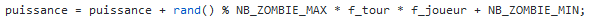
\includegraphics[width=\textwidth] {puissance.PNG}
La variable \textit{puissance} est la puissance de l'attaque, la variable \textit{f tour} est le nombre de tour sous format float, la variable \textit{f joueur} est le nombre de joueur sous format float et le \textit{rand()} est évidemment la valeur aléatoire. \textit{NB ZOMBIE MAX} et \textit{NB ZOMBIE MIN} sont des constantes faites pour que la puissance ne soit ni trop grande ni trop petite. Elles valent respectivements deux cent cinquantes et dix.

\newpage

\subsubsection{Implémentation réseau}

Ensuite nous allons voir l'intéraction entre le serveur et le client.
\begin{figure}[h]
    \begin{center}
    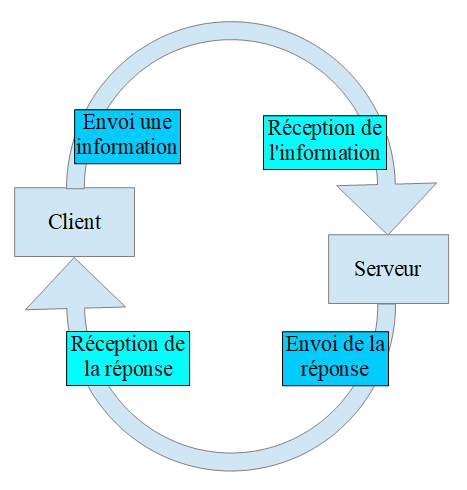
\includegraphics[width=\textwidth] {socket.PNG}
    \caption{Schéma montrant l'intéraction entre le client et le serveur}
    \label{reseau}
    \end{center}
\end{figure}

Pour faire simple, le module client possède le menu d'affichage dans lequel le joueur va pouvoir faire une action. Lorsque le joueur entre dans le menu pour la première fois, le menu lui demande son nom puis va mettre la chaine de caractère contenant son nom dans une variable appelée \textit{buffer} pour l'envoyer dans le module serveur. Le serveur possèdant maintenant le nom du joueur va pouvoir le créer et écouter les prochaines commandes qu'il fera. Après avoir choisi une action le module client envoi cette information au serveur qui lui va donner une réponse suivant l'action. Ainsi toutes les variables, structures sont entièrement gérer du côté serveur, alors que le côté client n'a à s'occuper que de l'affichage du menu. Les fonctions nécessaires au fonctionnement du système sont :
\\
\\
- socket() : cette fonction va créer une socket, c'est l'identifiant utilisé dans le système.
\\
\\
- bind() : cette fonction va assigner une adresse dans la mémoire pour la socket.
\\
\\
- listen() : cette fonction permet de voir les connections entrantes.
\\
\\
- accept() : cette fonction va accepter la connexion entrante.
\\
\\
- send() : cette fonction est utilisée pour envoyer un message.
\\
\\
- recv() : cette fonction est utilisée pour recevoir un message.

\subsubsection{La struture joueur et la liste des joueurs}

Abordons maintenant la structure joueur. La structure joueur et les fonctions liées sont définies dans le module joueur. La structure est composé du nom du joueur, son nombre de PA, un tableau de quatre pointeurs qui pointent chacun sur un objet, un tableau d'entier servant pour les états de santé, d'un entier indiquant les défenses de la maison, une liste d'objet correspondant à son coffre et ses coordonnées géographiques (x et y). Nous utilisons aussi un enum dans le tableau de santé pour éviter d'utiliser des nombres dans les fonctions. Les principales fonctions du module permettent de consulter la structure, par exemple voir l'inventaire du joueur. Il existe aussi une fonction pour créer le joueur et une autre pour supprimer le joueur.
\\

La liste de joueur est une liste contenant tous les joueurs connectés au serveur. On la parcours avec les primitives de la liste comme vu en cours. Chaque élément de la liste est un pointeur sur une structure joueur. Une fonction permet de voir d'afficher le nom de tous les joueurs ainsi que leur inventaire. Une autre permet de trouver un joueur en regardant le nom, cette fonction permet au module client de n'avoir à connaitre que le nom du joueur pour fonctionner.

\newpage

\subsection{Carte et Action extérieur}

Dans cette partie consacrée à la grande porte nous allons parler du développement de tout ce qui tourne autour de ce module que nous pourrons séparer en trois parties. La première concernera la création de la matrice correspondant à la carte, la seconde portera sur tous les changements concernant la carte pour chaque nouvelle journée et la dernière partie sera sur les actions du joueur sur la carte.

\subsubsection{Création de la matrice}

La carte est composée de 13 cases par 13 cases. Comme nous pouvons le voir dans le fichier case.h, chaque case, nommée case t, est composée d’un état de la case, si cette dernière a été fouillée ou non et si elle comporte ou non des zombies. Ensuite nous avons son état de fouille, si la case a été fouillée ou non, pour savoir par la suite si un joueur pourra la fouiller ou non. Ensuite nous avons une liste d’objet qui correspond aux objets présents sur le sol de cette case. Nous avons aussi le nombre de zombie ainsi que le nombre de joueur présent sur cette case. Pour allouer la mémoire de cette carte on créer toutes les cases une par une avec deux boucles imbriquées pour les colonnes et les lignes. Cette fonction de création de carte est générique, c’est-à-dire qu’elle peut être utilisé par n’importe qui pour allouer la mémoire d’une carte, on a juste à lui donner les dimensions de la carte que l’on souhaite et mettre à disposition un fichier case.h avec la structure de case qui nous convient. Une fois que la mémoire est allouée, on parcourt toute la carte pour mettre ce qui compose la carte à leur état initial. Pour finir avec l’initialisation de la carte, on place la ville au centre de la carte. Pour finir sur cette partie nous pouvons indiquer la présence de la fonction qui permet de libérer la mémoire de la matrice dans le module matrice.c.

\subsubsection{Changements dans la carte}

Nous allons maintenant nous attarder sur la fonction de tour de jeu. Cette fonction est appelée à chaque fois que l’attaque de zombie à lieu dans le thread du main. Au début de la fonction, nous explorons toute la carte avec deux boucles imbriqué pour remettre toutes les cases, si ça n’est pas la ville, à leur état initial. Ensuite nous parcourons la liste de joueur et si un joueur a ses coordonnées différentes à celles de la ville, la fonction appelle une autre fonction permettant de « tuer » le joueur c’est-à-dire de l’ôter de la partie. Ensuite viens la partie où l’on place les zombies sur la carte pour la nouvelle journée. Pour savoir combien de zombie nous allons avoir sur la carte, on demande lors de l’appel de la fonction un nombre correspondant aux nombre de jours et le nombre de zombie qui étaient présents sur la carte la veille. Grâce à une fonction logarithme et en fonction du nombre de jour et du nombre de zombie on détermine le nombre de zombie à placer sur la carte. Après on place les zombies un par un aléatoirement sur la carte en vérifiant que ça n’est pas la position de la ville sans oublier d’ajouter le nombre de zombie à la case donnée.

\subsubsection{Actions sur la carte}

Pour la partie concernant les actions, quand dans le menu du main on appelle la grande porte, nous arrivons dans un autre menu où l’on choisis les actions que l’on veut effectuer.
\\
\begin{figure}[h]
    \begin{center}
    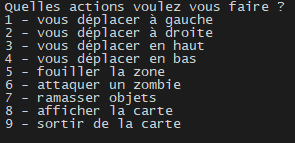
\includegraphics[width=8cm] {choix_carte.png}
    \caption{Affichage terminal des choix}
    \label{choix}
    \end{center}
\end{figure}

On a tout d’abord les fonctions de déplacement gauche, droite, haut et bas. Comme on peut s’en douter ses quatre fonctions sont très similaires. Au début de ces fonctions, on vérifie que le joueur a toujours des PA (points d’actions), on vérifie ensuite que le joueur ne veut pas se déplacer hors de la carte. Si toutes les conditions sont respectées, on déplace le joueur sans oublier de soustraire par un le nombre joueurs présents à la case précédentes et d’ajouter un à la nouvelle position du joueur. On regarde ensuite l’état de la case à la position du joueur. Si la case a son état non exploré alors on regarde s’il y a des zombies, si c’est le cas on met l’état de la case à explorée avec des zombies, sinon on met l’état en exploré neutre. On enlève ensuite un PA au joueur.
On a par la suite la fonction qui permet de fouilles la case où on est. Pour cette fonction on vérifie si le joueur est bien sur une zone qui n’as pas déjà été fouillée et qu’il n’est pas sur la position de la ville. On met l’état de fouille de la case a fouillée si le joueur a respecté les conditions. On détermine ensuite aléatoirement le nombre d’objet que l’on va trouver entre 1 et 4. Ensuite pour chaque objet on détermine ce que c’est encore une fois aléatoirement et on l’ajoute à la liste d’objet de la case.
Pour la fonction attaquer on vérifie que le joueur a encore des PA, qu’il est sur une case où il y a des zombies et qu’il n’est pas blessé. Une fois ces conditions réunies, on réduit le nombre de zombie et s’il est à zéro après ça on change l’état de la case pour le mettre en neutre. On réduit ensuite le nombre de PA du joueur par un. Le joueur a désormais une chance sur quatre d’avoir été blessé lors de cette confrontation.
Pour la fonction de ramassage d’objet, on vérifie d’abord que le joueur n’a pas son inventaire plein. On affiche alors la liste des objets au sol puis on demande ce qu’il désire mettre dans son inventaire. Une fois son choix fait on parcours la liste pour retirer l’objet de la liste d’objet de la case et de le mettre dans l’inventaire du joueur.
Les fonctions poser et utiliser font respectivement appel aux fonctions deposer objet et utiliser objet du module action.c.
\\
\begin{figure}[h]
    \begin{center}
    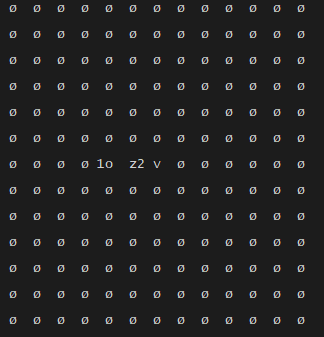
\includegraphics[width=8cm] {carte.png}
    \caption{Affichage terminal de la carte}
    \label{carte}
    \end{center}
\end{figure}

La fonction afficher carte a pour but, comme vous vous en doutez, d’afficher la carte. Voici ci-dessus le rendu que nous avons. La fonction parcourt toute la carte et regarde les caractéristiques de la case. Nous pouvons voir sur une grande partie de la carte des ronds barrés. Ces ronds correspondent à l’état non exploré. Ensuite nous pouvons voir un rond avec un 1 à sa gauche. Le 1 correspond aux nombres de joueurs présents sur la case et le rond correspond à l’état exploré neutre. A côté de cette même case, nous voyons un z avec un deux à sa droite. Le z veut dire que c’est une case avec des zombies dessus et le deux correspond aux nombre de zombies présents. Le v au milieu de la carte correspond à la case de la ville.
Nous avons une dernière fonction nommée sortir. Cette fonction vérifie que nous sommes aux coordonnées de la case pour pouvoir sortir de la grande porte et revenir au menu principal.

\newpage

\subsection{Objets et Batiments}

\subsubsection{Implémentation des objets}

Ils existent plusieurs catégories d'objets :
\\
\\
La nourriture : Cette catégorie d'objet permet aux joueurs de récupérer des points d'actions .
\\
\\
Les armes : Elles permettent aux joueurs de tuer des zombies en dehors de la zone sans utiliser de points d'actions.
\\
\\
La drogue : Cet objet spécial permet d'annuler les états de fatigue, et de regagner des points d'actions malgré la règle qui interdit de récupérer des points d'actions une fois que l'on a bu et manger.
\\
\\
Les transformables : Ceux-là sont des des objets qui permettent de fabriquer des matériaux.
\\
\\
Les matériaux : Composés de transformables, ils permettent de créer des défenses contre les zombies.
\\
\\
Les objets sont représentés par une structure avec leurs noms, catégories, descriptions, et attribut ( défini par une structure union).
\\
\\
Tout les objets existants sont dans une liste et sont récupérés à l'aide d'un fichier texte contenant tout les objets. La liste est mise en œuvre par des pointeurs et plusieurs listes d'objet peuvent être créer.

\newpage

Comment l'objet circule au niveau des bâtiments :
\begin{figure}[h]
    \begin{center}
    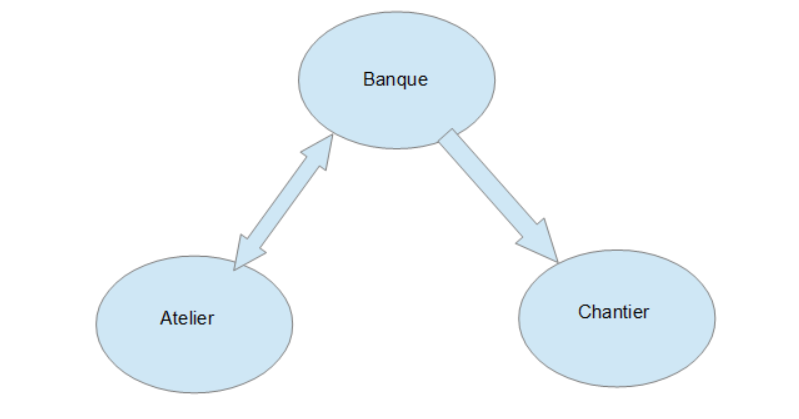
\includegraphics[width=\textwidth] {objet.PNG}
    \caption{Schéma du cycle de l'objet}
    \label{objet}
    \end{center}
\end{figure}

\subsubsection{Implémentation des bâtiments}

Le puit : Ce bâtiment permet aux joueurs de récupérer une ration d'eau pour récupérer des points d'actions. Les rations d'eau sont limités et sont définis à 150 au début de la partie, le joueur peut donc soit prendre de l'eau si son inventaire le permet, soit en ajouter afin de partager de l'eau avec les joueurs en difficulté.
\\
\\
La maison : Elle sert de zone de repos pour le joueur, elle possède un coffre (une liste d'objets) avec lequel le joueur peut gérer son inventaire afin de choisir quel objet stocker, ou quel objet récupérer. Cette zone permet au joueur d'effectuer l'action crucial de manger ou boire qui ne s'effectue que dans cet endroit ou en dehors de la ville. Enfin le joueur peut décider d'améliorer sa maison ce qui diminuera ses chances de mourir lors d'une attaque de zombie, mais cet action nécessite des points d'actions. La défense de la maison est représenté par un entier défini dans la structure joueur.
\\
\\
La banque : C'est la zone de partage d'objets, elle possède un inventaire illimité. Les joueurs peuvent soit déposer des objets de leurs inventaire, soit en prendre à la banque. La banque sert aussi à approvisionner l'atelier en transformable, et le chantier en matériaux. Au niveau du code la banque est représenté par une structure qui contient plusieurs listes d'objets , ces listes stockent les objets selon leurs catégories . Au début du jeu ces listes sont initialisés, afin que la banque soit fonctionnelle les joueurs doivent impérativement déposer des objets sinon elle perd son utilité. Lorsque qu'un joueur entre dans la banque un menu s'affiche à l'aide d'un switch, lui proposant d'afficher les objets de la banque et son inventaire, de déposer ou de prendre un objet. Les actions tel que prendre un objet proviennent du module action, cela permet d'alléger le code et de l'utiliser dans les différents modules.
\\
\\
L'atelier : Le rôle de ce bâtiment est de mettre en place un assembleur d'objet, en dehors de la ville des objets de la catégorie transformable peuvent être récupérer, en les déposant dans la banque le joueur peut utiliser l'atelier afin de créer des matériaux. Ces matériaux lui permettront de créer des défenses qui permettront de repousser ou non(selon leurs nombres) l'attaque de zombie. Le joueur doit seulement prendre l'objet est effectuer l'action de transformation et perdre un peu de ses points d'actions. Le matériau une fois construit se place automatiquement dans la banque et est prêt à être utiliser dans le chantier.
\\
\\
Le chantier : Les défenses contre les zombies proviennent de ce bâtiment, les matériaux précédemment construits peuvent être utilisés afin de créer ces défenses . Les défenses sont définis par une structure qui contient le nombre de défense qui sera attribué à la ville si la défense est construite, les points d'actions nécessaire pour la construction, les matériaux et le nombre nécessaire à chacun et son statut afin de savoir si la défense à déjà été construite. Une liste a été créer pour pouvoir stocké les défenses qui seront  récupérer sur un fichier texte. Lorsque le joueur arrive sur le chantier on peut afficher les défenses disponible, pour cela on parcours la liste est on affiche uniquement les défenses non construites. Le joueur peut alors choisir de dépenser un nombre de points d'actions dans une des défenses. 

\newpage

\section{Résultats}
Au cours de ce projet nous avons réalisé un grand nombre de nos objectifs fixés même si nous n’avons malheureusement pas implémenter tout ce que nous pouvons faire mais nous avons malgré tout atteint nos objectifs principaux qui sont les suivants. Pouvoir avoir un jeu jouable en version terminale et pouvoir jouer en réseau.
\\

Nous avons donc fourni une version terminale du jeu en réseau avec la possibilité d’aller dans chaque module et dans chaque endroit la possibilité d’interagir avec le lieu. Nous avons donc la possibilité d’accéder à sa maison, de prendre de l’eau au puits et d’interagir avec la banque, le chantier et l’atelier et d’accéder à l’extérieur de la carte et encore une fois d’interagir avec. Nous avons aussi une version avec le réseau quasi fonctionnel où nous avons un serveur et plusieurs clients avec pour chaque client un terminal à ouvrir.  
Voici un exemple de connexion au serveur puis de déconnexion depuis un client.
\\
\begin{figure}[h]
    \begin{center}
    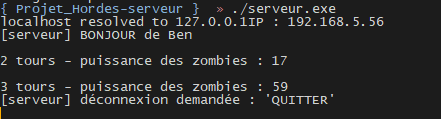
\includegraphics[width=8cm] {res1.png}
    \caption{Exemple connexion serveur}
    \label{serveur}
    \end{center}
\end{figure}

Nous avons ici la version du client
\\
\begin{figure}[h]
    \begin{center}
    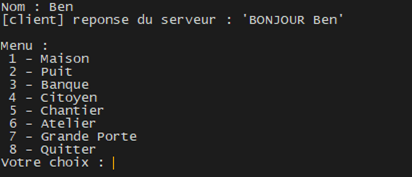
\includegraphics[width=8cm] {res2.png}
    \caption{Exemple connexion client}
    \label{client}
    \end{center}
\end{figure}

Au cours de ce projet nous n’avons malheureusement pas eu le temps d’implémenter une partie graphique autre que le terminal avec la librairie SDL mais ça n’était pas notre priorité.


\newpage

\section {Conclusion}
Pour conclure, ce projet a été une expérience extrêmement enrichissante, il nous a permis de mieux travailler et de collaborer en équipe, d'améliorer nos connaissances en programmation, d'apprendre de nouvelles façons de programmer, notamment avec Github. Ce projet nous a donné un échantillon de ce qui nous attendra lorsque nous programmerons au sein d'une société.
\\
\\
Ce projet peut encore être amélioré si nous avions plus de temps et de moyen. Parmi les ajouts possibles, nous aurions pu implémenter d'autres aspects présents dans le jeu original, par exemple les classes héros.

Les héros sont des joueurs qui ont des fonctionnalités spéciales suivant leur classe, certains peuvent par exemple se téléporter dans la ville alors qu'ils sont à plusieurs cases de celle-ci sans coût en PA. Nous avons estimé que ses classes n'apportaient que des inégalités au jeu, les joueurs non héros étant désavantagés. De plus les classes héros nécéssitent de payer un certain montant pour pouvoir être jouer dans le jeu original, nous avons donc pas vraiment pu voir toutes les possibilités de ces classes.

Un autre aspect du jeu original est la présence de goule au sein des citoyens. Les goules sont des citoyens (donc joueur) qui peuvent tuer puis manger d'autres citoyens. Ils peuvent survivre en dehors de la ville et leur but est donc d'être le dernier survivant (une goule pouvant manger une autre goule). Cette fonctionnalité ne rentrait pas très bien dans le cadre d'un jeu en réseau local, tout simplement car le nombre de joueur est moins grand que dans le jeu original et aussi car le réseau local se prête plus à la coopération plutôt qu'à la trahison.

Enfin il reste aussi les objets et infrastructures que nous n'avons pas implémenté car il y en a trop et beaucoup se ressemble.

\newpage

\end {document}